\documentclass[11pt, oneside]{article}   	% use "amsart" instead of "article" for AMSLaTeX format
\usepackage{geometry}                		% See geometry.pdf to learn the layout options. There are lots.
\geometry{letterpaper}                   		% ... or a4paper or a5paper or ... 
%\geometry{landscape}                		% Activate for for rotated page geometry
%\usepackage[parfill]{parskip}    		% Activate to begin paragraphs with an empty line rather than an indent
\usepackage{graphicx}				% Use pdf, png, jpg, or eps� with pdflatex; use eps in DVI mode
								% TeX will automatically convert eps --> pdf in pdflatex		
\usepackage{amssymb}
\graphicspath{{/Users/telliott_admin/Dropbox/Tex/png/}}

\title{Sine and cosine of simple angles}
%\author{The Author}
\date{}							% Activate to display a given date or no date

\begin{document}
\maketitle
%\section{}
%\subsection{}
\setlength{\parskip}{2 mm}
\large
We'll consider the two simple triangles shown below.  
\begin{center}
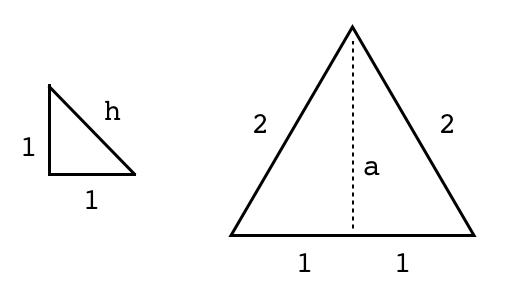
\includegraphics [scale=0.5] {simple_tri.png}
\end{center}
The one on the left is a right triangle with both side lengths equal to 1.  Since it is an isosceles triangle, the two angles that flank the hypotenuse are equal.  Since the sum of those angles is $90^\circ$, each one is $45^\circ$.

Furthermore, by the Pythagorean theorem $h^2 = 2$ so $h=\sqrt{2}$.  Therefore
\[ sin(45^\circ) = cos(45^\circ) = \frac{1}{\sqrt{2}} \]
Or, using radians for the angle measure:
\[ sin \frac{\pi}{4} = cos \frac{\pi}{4} = \frac{1}{\sqrt{2}} \]
The triangle on the right is an equilateral triangle.  If we drop an altitude a, the two smaller triangles are congruent.  Since both are right triangles and the angles at the base (left and right) are $60^\circ$, these are 30-60-90 triangles.  The angles at the top are both equal to $30^\circ$, so we see that
\[ sin(30^\circ) = cos(60^\circ) = \frac{1}{2} \]
Using radians for the angle measure
\[ sin(\frac{\pi}{6}) = cos(\frac{\pi}{3}) = \frac{1}{2} \]
We can find the length of $a$ by the Pythagorean Theorem, it is equal to $\sqrt{3}$.  So the cosine of $30^\circ$
\[ cos(30^\circ) = cos(\frac{\pi}{6}) = sin(60^\circ) = sin(\frac{\pi}{3})=  \frac{\sqrt{3}}{2} \]


Finally, let's do $22.5^\circ$
\begin{center}
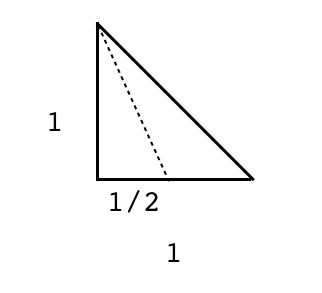
\includegraphics [scale=0.5] {22_5.png}
\end{center}
While the figure above looks tempting, it is not correct!  $tan^{-1}(1/2) = 26.565^\circ$.

\begin{center}
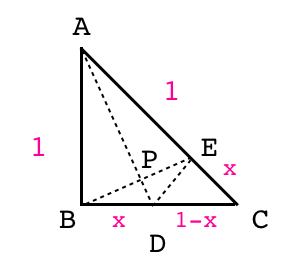
\includegraphics [scale=0.5] {fancy_tri.png}
\end{center}

We draw $AP$, the bisector of $45^\circ$ $\angle BAC$ and also draw $BE$, a perpendicular to the bisector, as shown.  $BE$ divides the hypotenuse into two pieces.  Now we have an isosceles $\triangle ABE$ with sides of 1 and an apical angle of $45^\circ$, so the angle $\angle ABP$ at its base is $67.5^\circ$.

We also connect the two new points $DE$.

Since $\angle APE$ is a right angle, and $AP$ is the angle bisector, $\triangle APB \cong \triangle APE$, by $AAA$ plus one side (all four angles at $P$ are right angles).  Therefore, $BP = PE$.
\vspace{2 mm}

By $SAS$, $\triangle BPD \cong \triangle DPE$.  Therefore, $DE = BD = x$.
\vspace{2 mm}

Also, $\angle BAP$ and $ABP$ add to $90^\circ$, but so do $\angle ABP$ and $\angle PBD$, so $\angle PBD = \angle BAP$, and the two pairs of triangles are all similar.
\vspace{2 mm}

Finally, since $\triangle APE \sim \triangle DPE$, $\angle AEP$ and $\angle PED$ are complementary and so $\angle AED = \angle DEC$ is a right angle.  Since $\angle DCE = 45^\circ$, $\angle EDC = 45^\circ = \angle DCE$  and thus, $\triangle DEC$ is isosceles, and $EC$ is also equal to $x$.

\begin{center}
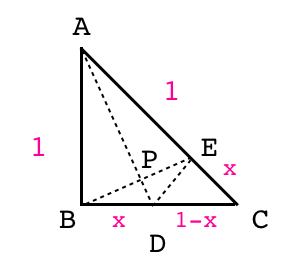
\includegraphics [scale=0.5] {fancy_tri.png}
\end{center}

We look at the figure again and focus on the side lengths.  From $\triangle DEC$ we see that 
\[ \frac{x}{1-x} = cos(45^\circ) = \frac{1}{\sqrt{2}} \]
Inverting we have
\[ \frac{1-x}{x} = \sqrt{2} \]
\[ \frac{1}{x} = 1 + \sqrt{2} \]

\[ x = \frac{1}{1 + \sqrt{2}} \]
From $\triangle ABD$ we see that 
\[ x = \frac{1}{1 + \sqrt{2}} = \frac{1}{2.414} = 0.4142 =  tan(22.5^\circ) \]
And this can be easily checked on a calculator.  To get the sine and cosine requires computing the hypotenuse.

\subsection*{a better way}
However, after all that, I must admit there is another way.  It involves the formula for sum of cosine
\[ cos(s+t) = cos \ s \ cos \ t - sin \ s \ sin \ t \]

If $s=t$
\[ cos(2s) = cos^2s - sin^2s = 2cos^2s - 1 \]
\[ cos^2s = \frac{1}{2}(1 + cos(2s)) \]
\[ cos\ s = \sqrt{\frac{1}{2}(1 + cos(2s))} \]
since
\[ cos(45^\circ) = cos(2s) = 1/\sqrt{2} \]
\[ cos \ s = cos(22.5^\circ) = \sqrt{\frac{1}{2}(1 + \frac{1}{\sqrt{2}})} = 0.9239 \]
\[ sin(22.5^\circ) = \sqrt{1-cos^2(22.5^\circ)} =  \sqrt{1-(0.9239)^2} = 0.3826 \]

And in general, the full complement of sum and difference equations
\[ sin(s+t) = sin \ s \ cos \ t + sin \ t \ cos \ s \]
\[ sin(s-t) = sin \ s \ cos \ t - sin \ t \ cos \ s \]
\[ cos(s-t) = cos \ s \ cos \ t = sin \ s \ sin \ t \]

can be used to obtain sine and cosine for other angles, starting with these four (plus $90^\circ$).  We can get $15^\circ$ as half of $30^\circ$ and $7.5^\circ$ as half of $15^\circ$, or as the difference between $30^\circ$ and $22.5^\circ$.

\end{document}
